\section{Evaluation Plan}
\label{sec:eval-plan}
% \todo{note for evaluation, section on real-life testing and simulation tsting separately, to observe potential differences}
% As the project is an evaluation of the proposed framework upon adding active vision elements. It will have to be done on a pre-set collection of robot tasks. 
% Firstly, these tasks will be attempted with conventional approaches as control, either pre-trained open-sourced policies in a static-camera setting, or in-house policies without active perception. This will show us whether the improvements we suggest, in the form of extra learning and acting through active vision, has an affect on the success rate of the agents learning to do these tasks.

% On top of in-simulation testing, the 

I am currently planning to evaluate the policies I train on RLBench \cite{james2019rlbenchrobotlearningbenchmark}. A public benchmark designed for reinforcement learning algorithms and uses CoppeliaSim \cite{CoppeliaRobotics} in the backend.

CoppeliaSim is a mostly open-sourced, allowing the aforementioned RLBench, which is essentially a python wrapper to provide easy and programmatic access to the simulation environment. Also, in the long-run its realistic physics and rendering might allow our models trained there to be deployed in real-world environments, though will require additional verifications and the tests will not initially designed to accommodate this.

\subsection{Policy Performance}
The main focus of this project is to propose methods of active learning that are at least as good as static camera models in all scenarios and at least somewhat better (within the testing criteria) given some uncertainty for us to conclude whether active vision is a topic worth exploring.

\subsubsection{Baseline Evaluation}
Therefore, we need to establish some baseline policy performance, to be able to compare the outcomes of tasks. Some information we can evaluate are:
\begin{itemize}
  \item \textbf{Success Rate:} Percentage of times where the given scenario was executed correctly. Judged either by eye manually, or by some mechanism in the setup.
  \item \textbf{Failure Rate:} Similarly, ratio of runs where the policy doesn't complete the task satisfactorily
  \item \textbf{Time to Completion:} Mean time a policy, along many runs, takes to complete a task. 
  \item \textbf{Efficiency:} This will have to be explored to find what ``efficient'' would mean in the context of a benchmark. However, it could mean things like, how many steps to complete a reach-the-target sort of task (action efficiency), or path efficiency based on distance traveled to target etc.
\end{itemize}
These metrics will allow us to compare the active vision system proposed to baselines with different mounted camera positions.

\subsubsection{Inter-Active Benchmarks}
As we are planning on proposing multiple active learning policies, we should also have a method to compare them between each other. This comparison can use metrics such as:
\begin{itemize}
  \item \textbf{Camera Movement:} How much the camera moves in finding better viewpoints, can be expressed in terms of the total magnitude of movement at the end of an episode or run.
  \item \textbf{Frequency of View Changes:} This could give an insight into the policies \emph{sureness} or decision capability, choices that change the viewpoint frequently may hint at robustness issues.
  \item \textbf{Uncertainty Reduction:} Similar to above, as these policies are actively trying to decrease uncertainty in the given scene, it might be a good performance comparison to see entropy changes per model.
  \item \textbf{Occlusion Avoidance:} As this is one of the main topics advocating for active vision, we must characterise the performance of a model to avoid getting itself behind obstacles that might occlude goals. This might be defined in relation to the last two points covered above, or defined per task depending on the level of occlusion we place in a scene.
  \item \textbf{Success Rate in Occluding Scenarios:} Another follow-up point, using purposefully engineered tests that include multiple levels of occlusion, what success ratios can different models achieve. 
  \item \textbf{Novel Adaptation:} Comparing performance characteristics of completion of a task in different settings (such as different backgrounds) could give good insight about training scene generalisation. Or starting the robot in poses not demonstrated to check viewpoint novelty could give us good insight about a policy.
  \item \textbf{Noise Performance:} Similar to above, we can also experiment with noise such as varying lighting levels of the scene or different textures on objects to see if these can cause more failures and whether active perception will tackle random noise addition.
  \item \textbf{Simulation to Real Life:} Finally, if the project gets to the level of using these models in real-life, we can tests for the sim-to-real robustness and transferability of a policy by making it to the same tests in the simulation and real life and comparing some of these defining characteristics.
\end{itemize}

\subsubsection{Resource Utilisation}
Another section of the testing might include the acting performance of an agent compared to its computational performance. We can compare: \textbf{inference times}, \textbf{latencies is switching policies} between vision and motor (physical action) and maybe even \textbf{computational load} or \textbf{resource usage} depending on the architecture and its complexity. This might give us insight into the \emph{costs} of a performant policy.

\subsection{Initial Evaluation Proposal}
Although, we cannot create the entire benchmarking suite at this time, the general guidelines above will help us create a set of tasks that accurately assess the performance characteristics of our models. However, the suggestions above are in no way final and more can be added or some removed depending on relevancy of application to the test or benchmark.

\subsubsection{Basic Proposed Tasks}
As we are mainly concerned about active vision our tasks should include:
\begin{enumerate}
  \item \textbf{Navigation:} A path finding or reaching task differing levels of difficulty, such as: no obstacles, some obstacles to overcrowded and complex environments.
  \item \textbf{Grasping:} A classical example of a task we can explore the performance of a grasping task with policies such as eye-in-hand and a grasping task where the camera is decoupled from the gripper, but still active.
  \item \textbf{Searching:} This could be an interesting task, to test the limits of understanding coupled with a robots active abilities, for example searching for a ``red ball'' in a drawer of balls
\end{enumerate}

\subsubsection{In Simulation}
These tasks might look like the following in Figure \ref{fig:threesims}.
\todo{enter some pictures from the siumulation for a basic nav, grasp and searching task}

\begin{figure}[h]
  \centering
  \begin{minipage}{0.32\textwidth}
    \centering
    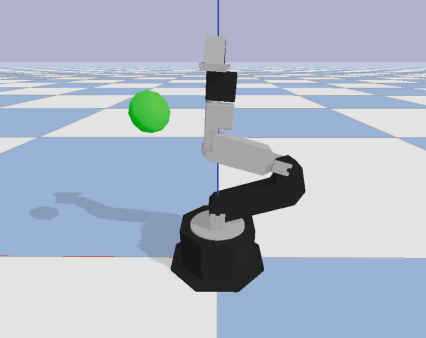
\includegraphics[width=\textwidth]{assets/eval-plan/reach-sim.png}
    \caption{Simple Simulated reaching task made in pybullet where the green orb is the target area, taken from \cite{aumjaud2020reinforcement}}
  \end{minipage}
  \hfill
  \begin{minipage}{0.32\textwidth}
      \centering
      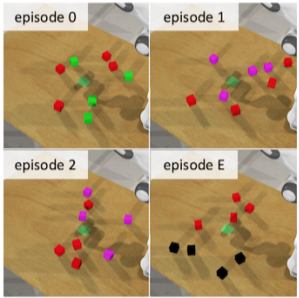
\includegraphics[width=\textwidth]{assets/eval-plan/grasp-sim.png}
      \caption{An example grasping task from RLBench \cite{james2019rlbenchrobotlearningbenchmark}}
  \end{minipage}
  \hfill
  \begin{minipage}{0.32\textwidth}
      \centering
      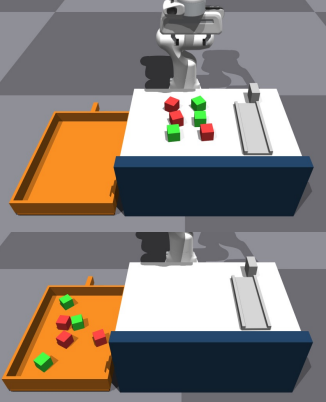
\includegraphics[width=\textwidth]{assets/eval-plan/search-sim.png}
      \caption{An example searching task from \cite{liang2022searchbasedtaskplanninglearned}}
  \end{minipage}
  \caption{Three Possible simulation tests, easiest level with no occlusions}\label{fig:threesims}
\end{figure}
